\documentclass[tikz,border=5pt]{standalone}
\usetikzlibrary{arrows.meta, backgrounds, fit, positioning}

\begin{document}
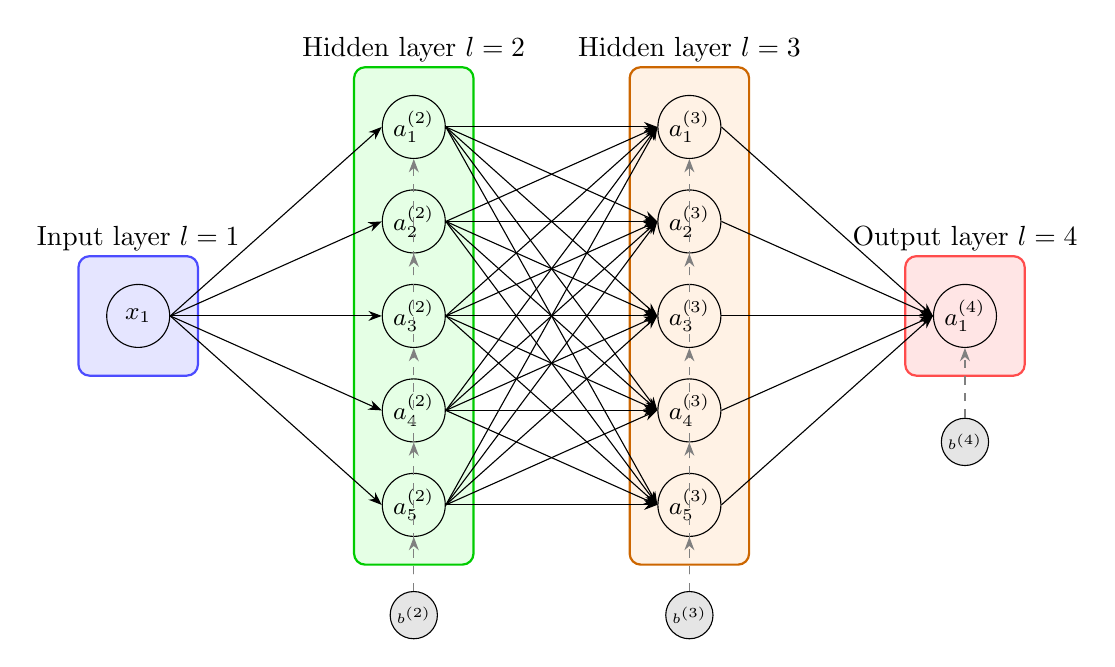
\begin{tikzpicture}[
    neuron/.style={circle, draw, minimum size=0.8cm, inner sep=0pt, font=\small},
    bias/.style={circle, draw, minimum size=0.6cm, inner sep=0pt, font=\tiny, fill=gray!20},
    >=Stealth,
    every edge/.style={draw, ->, thin}
]

% 输入层
\node[neuron] (x1) at (0,0) {$x_1$};
\node[above=0.3cm of x1] {Input layer $l=1$};

% 隐藏层1 (1-2-3-4-5 从上到下)
\foreach \i in {1,...,5} {
    \node[neuron] (a\i) at (3.5, {(3-\i)*1.2}) {$a_\i^{(2)}$};
}
\node[above=0.3cm of a1] {Hidden layer $l=2$};
\node[bias] (b2) at (3.5, -3.8) {$b^{(2)}$};

% 隐藏层2
\foreach \i in {1,...,5} {
    \node[neuron] (h\i) at (7.0, {(3-\i)*1.2}) {$a_\i^{(3)}$};
}
\node[above=0.3cm of h1] {Hidden layer $l=3$};
\node[bias] (b3) at (7.0, -3.8) {$b^{(3)}$};

% 输出层
\node[neuron] (y1) at (10.5,0) {$a_1^{(4)}$};
\node[above=0.3cm of y1] {Output layer $l=4$};
\node[bias] (b4) at (10.5, -1.6) {$b^{(4)}$};

% 全连接线
\foreach \j in {1,...,5} {\draw[->, thin] (x1.east) -- (a\j.west);}
\foreach \j in {1,...,5} {\draw[->, dashed, gray] (b2.north) -- (a\j.south);}
\foreach \i in {1,...,5} \foreach \j in {1,...,5} {\draw[->, thin] (a\i.east) -- (h\j.west);}
\foreach \j in {1,...,5} {\draw[->, dashed, gray] (b3.north) -- (h\j.south);}
\foreach \i in {1,...,5} {\draw[->, thin] (h\i.east) -- (y1.west);}
\draw[->, dashed, gray] (b4.north) -- (y1.south);

% 背景框
\begin{scope}[on background layer]
    \node[draw=blue!70, thick, rounded corners, fill=blue!10, fit=(x1), inner sep=10pt] {};
    \node[draw=green!80!black, thick, rounded corners, fill=green!10, fit=(a1)(a5), inner sep=10pt] {};
    \node[draw=orange!80!black, thick, rounded corners, fill=orange!10, fit=(h1)(h5), inner sep=10pt] {};
    \node[draw=red!70, thick, rounded corners, fill=red!10, fit=(y1), inner sep=10pt] {};
\end{scope}

\end{tikzpicture}
\end{document}